%\section*{\begin{center}{\Huge Appendix}\end{center}}
%\addcontentsline{toc}{chapter}{Appendix}
%$\\[0.5cm]$
\begin{appendices}
\chapter{Database statistics}

\begin{table}[h!]
\centering
\begin{tabular} {|| p{20em} | p{5em} ||} 
 \hline
 Category & Count \\ [0.5ex] 
 \hline
 Articles created via the Article Wizard & 86 \\
Articles containing video clips & 85 \\
Articles containing proofs & 76 \\
Ring theory & 74 \\
Protein domains & 73 \\
Linear algebra & 65 \\
Formal languages & 57 \\
Algebraic geometry & 53 \\
Living people & 51 \\
Naval guns of the United Kingdom & 51 \\
Commutative algebra & 50 \\
Game theory & 47 \\
Algebraic structures & 47 \\
Topology & 45 \\
Stochastic processes & 44 \\
Marketing & 44 \\
Functional analysis & 42 \\
Group theory & 42 \\
Coastal artillery & 42 \\
Combinatorics & 41 \\
Abstract algebra & 38 \\
Functional languages & 38 \\
Weather warnings and advisories & 36 \\
General topology & 36 \\
Management & 36 \\
Articles with example Java code & 36 \\
Victorian-era weapons of the United Kingdom & 36 \\
Signal processing & 35 \\
Category theory & 35 \\
Number theory & 35 \\
Social psychology & 34 \\
Architectural styles & 34 \\
Concepts in physics & 34 \\
1067 mm gauge locomotives of Japan & 34 \\
Algebra & 33 \\
 \hline
\end{tabular}
\caption{Statistics over most popular categories}
\label{table:A.1}
\end{table}

%%burde exemplene navngis av meg for refereing, ha hvert eksempen under en section?
%%burde jeg ha noen kilder?
\chapter{Example samples} \label{app_example}
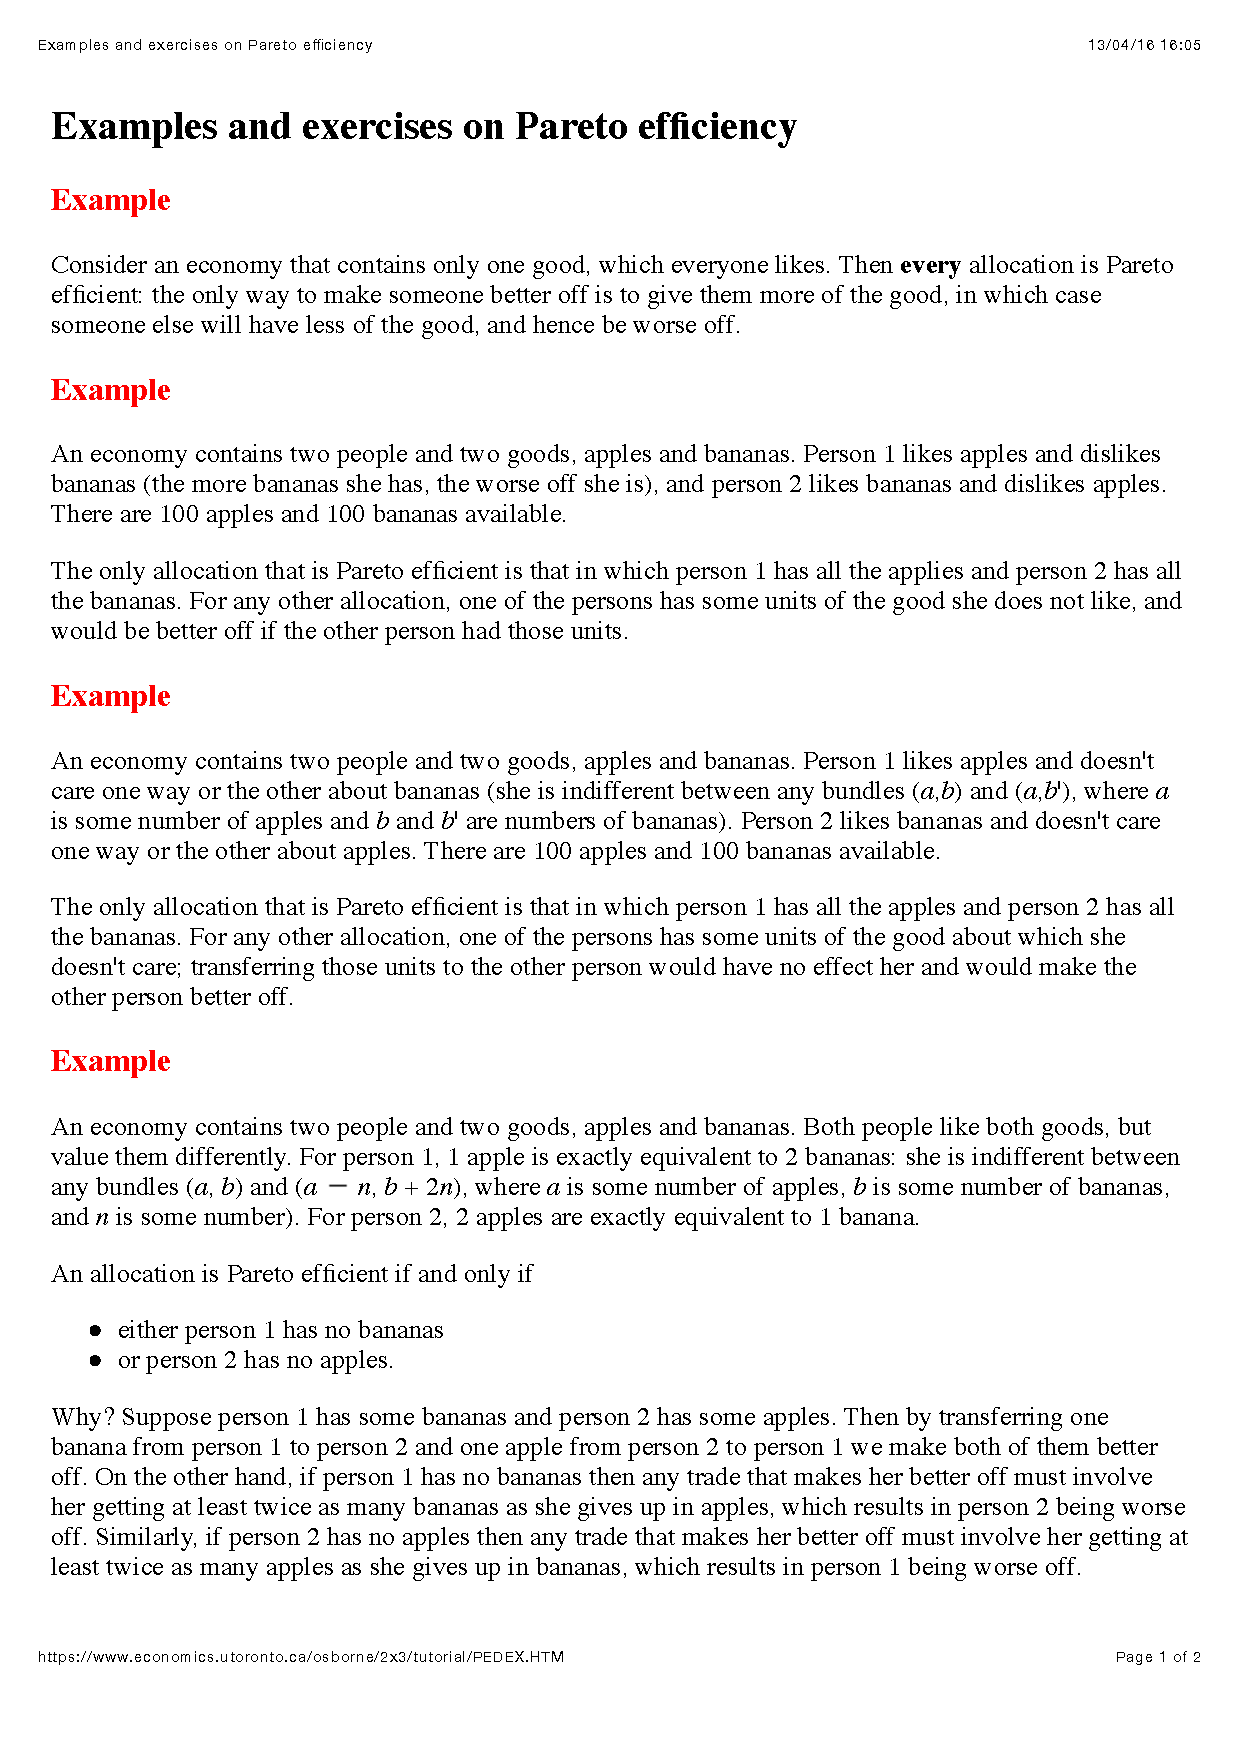
\includepdf[pages=-, scale=.8, pagecommand={}]{documents/pareto_example.pdf}
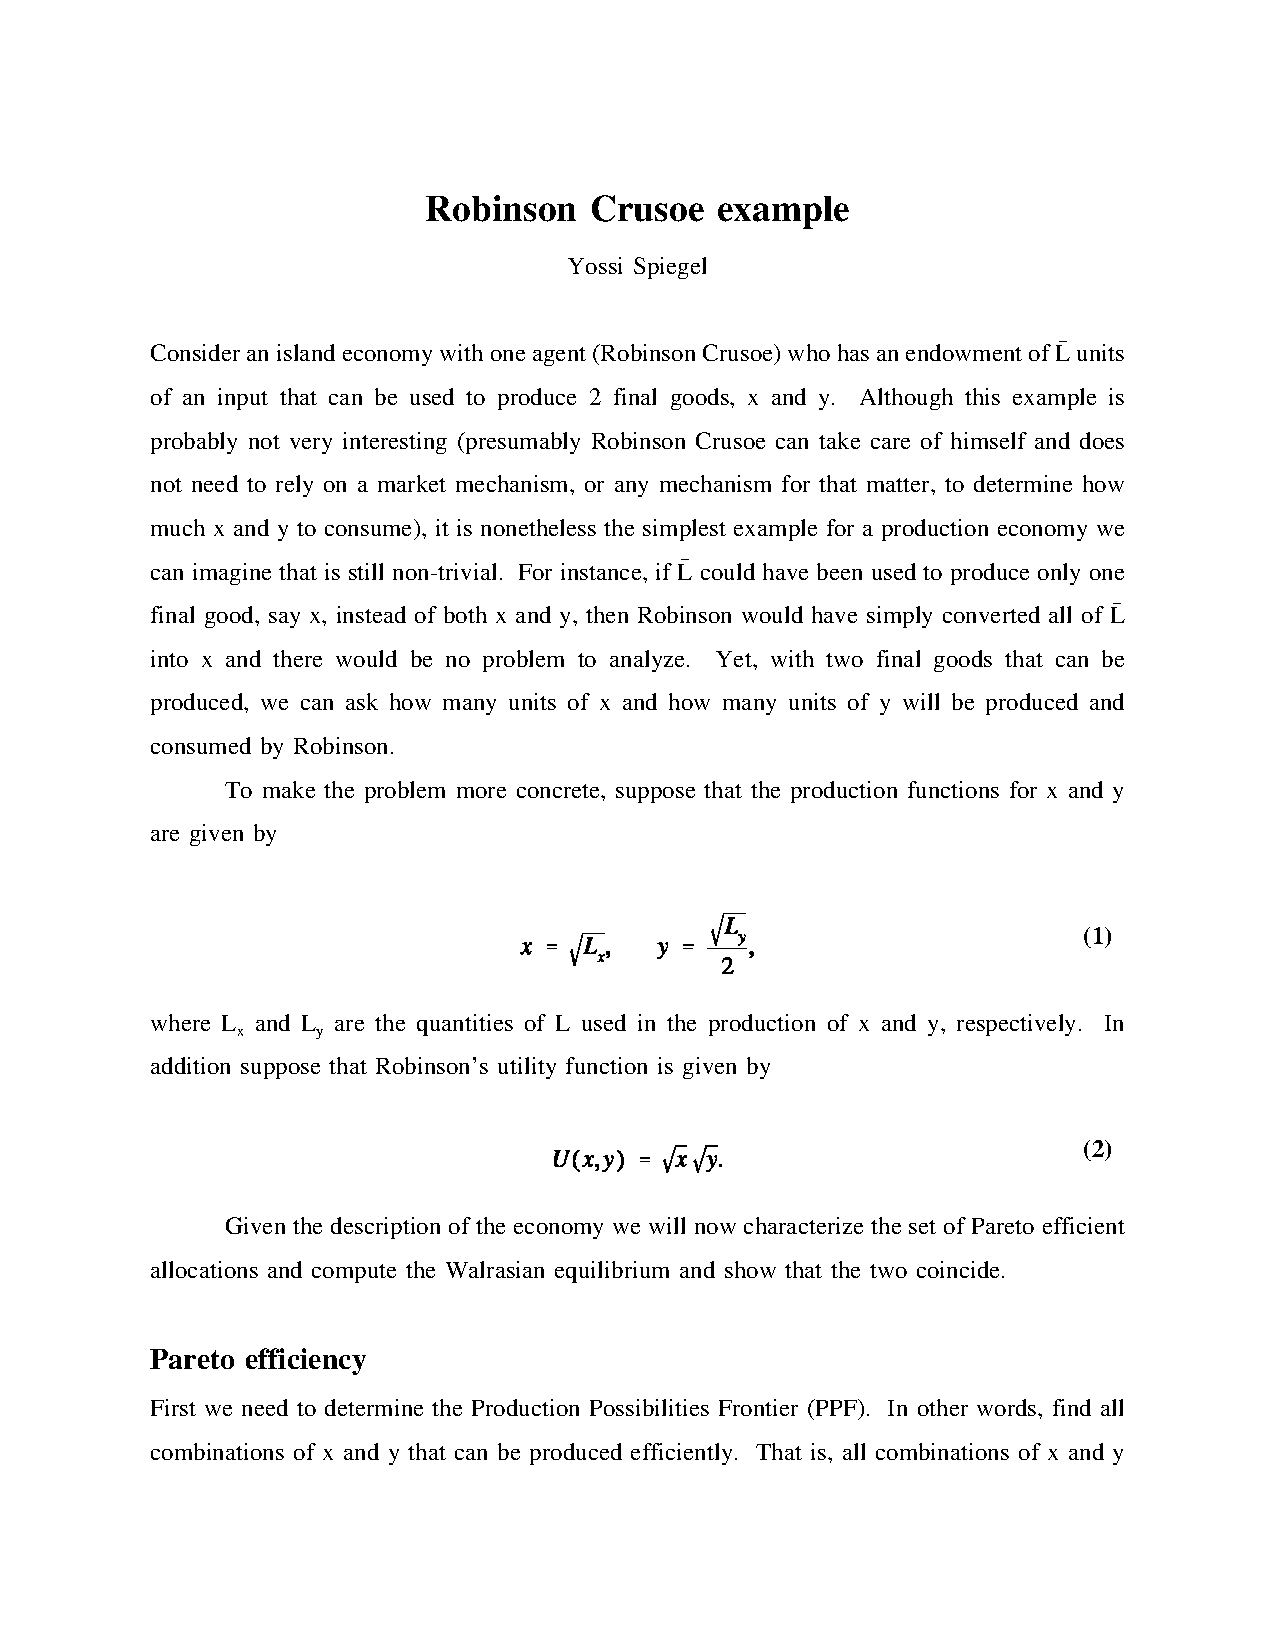
\includepdf[pages=-, scale=.9, pagecommand={}]{documents/Crueso.pdf}


\chapter{Example white lists} \label{app_whitelist}

\section{whitelist version 2}

\centering
\begin{longtable} {|| p{20em} | p{5em} ||} 
 \hline
 Category & Count \\ [0.5ex] 
 \hline
 
 Articles containing proofs	&	76	\\
Ring theory	&	74	\\
Protein domains	&	73	\\
Linear algebra	&	65	\\
Formal languages	&	57	\\
Algebraic geometry	&	53	\\
Commutative algebra	&	50	\\
Algebraic structures	&	47	\\
Game theory	&	47	\\
Topology	&	45	\\
Marketing	&	44	\\
Stochastic processes	&	44	\\
Group theory	&	42	\\
Functional analysis	&	42	\\
Combinatorics	&	41	\\
Abstract algebra	&	38	\\
Functional languages	&	38	\\
General topology	&	36	\\
Articles with example Java code	&	36	\\
Signal processing	&	35	\\
Category theory	&	35	\\
Number theory	&	35	\\
Concepts in physics	&	34	\\
Architectural styles	&	34	\\
Social psychology	&	34	\\
Algebra	&	33	\\
Polynomials	&	33	\\
Mathematical relations	&	33	\\
XML-based standards	&	33	\\
Object-oriented programming languages	&	33	\\
Dynamical systems	&	32	\\
Quantum mechanics	&	32	\\
Functions and mappings	&	32	\\
Statistical terminology	&	31	\\
Decision theory	&	31	\\
Genetics	&	30	\\
Model theory	&	30	\\
Ethology	&	30	\\
Articles with example pseudocode	&	30	\\
Procedural programming languages	&	30	\\
Mathematical optimization	&	30	\\
Probability theory	&	29	\\
Matrices	&	29	\\
Algebraic topology	&	29	\\
Properties of topological spaces	&	29	\\
Order theory	&	29	\\
Cross-platform software	&	28	\\
Estimation theory	&	27	\\
Integer sequences	&	27	\\
Protein families	&	27	\\
Field theory	&	27	\\
Semigroup theory	&	27	\\
Financial risk	&	26	\\
Fluid dynamics	&	26	\\
Molecular biology	&	26	\\
Measure theory	&	26	\\
Evolutionary biology	&	26	\\
Cryptography	&	26	\\
Properties of groups	&	25	\\
Combinatorics on words	&	25	\\
Semantics	&	25	\\
Statistical theory	&	25	\\
Metric geometry	&	25	\\
Cognitive biases	&	25	\\
Java platform	&	25	\\
Software design patterns	&	24	\\
Lie algebras	&	24	\\
Scripting languages	&	24	\\
Quantum field theory	&	24	\\
Differential geometry	&	24	\\
Representation theory	&	24	\\
Ecology	&	24	\\
Economics terminology	&	24	\\
Mathematical finance	&	23	\\
Control theory	&	23	\\
Mathematical logic	&	23	\\
Statistical models	&	23	\\
Theory of probability distributions	&	23	\\
Data management	&	23	\\
Binary operations	&	23	\\
Computer file formats	&	23	\\
Syntax	&	23	\\
Technical communication	&	23	\\
Software using the MIT license	&	22	\\
Object-oriented programming	&	22	\\
Numerical analysis	&	22	\\
Measures (measure theory)	&	22	\\
Software testing	&	22	\\
Mathematical analysis	&	22	\\
Diagrams	&	22	\\
Finance	&	22	\\
Graph families	&	22	\\
Classical mechanics	&	22	\\
Articles with example C++ code	&	22	\\
World Wide Web Consortium standards	&	22	\\
Architectural elements	&	22	\\
Data analysis	&	21	\\
Systems theory	&	21	\\
Bioinformatics	&	21	\\
Sociological terminology	&	21	\\
Computational complexity theory	&	21	\\
Homotopy theory	&	20	\\
Logic	&	20	\\
Module theory	&	20	\\
Markup languages	&	20	\\
Theory of computation	&	20	\\
Political terminology	&	20	\\
Partial differential equations	&	20	\\
Hydrology	&	20	\\
Matrix theory	&	20	\\
Linguistics	&	20	\\
Chess terminology	&	19	\\
E-commerce	&	19	\\
Parallel computing	&	19	\\
Physical quantities	&	19	\\
Educational psychology	&	19	\\
Legal terms	&	19	\\
Medical terminology	&	19	\\
Geometric group theory	&	19	\\
Artificial intelligence	&	19	\\
Epidemiology	&	19	\\
Algebraic number theory	&	19	\\
Numerical linear algebra	&	19	\\
Articles with example code	&	19	\\
Rhetoric	&	19	\\
Unix SUS2008 utilities	&	19	\\
Factorial and binomial topics	&	19	\\
Types of functions	&	19	\\
Knowledge representation	&	19	\\
Sociolinguistics	&	18	\\
Articles with example C code	&	18	\\
Digital signal processing	&	18	\\
Application programming interfaces	&	18	\\
Modular arithmetic	&	18	\\
Source code	&	18	\\
Graph algorithms	&	18	\\
Route diagram templates	&	18	\\
Mathematical physics	&	18	\\
Graph theory	&	18	\\
Equations	&	18	\\
Deception	&	18	\\
Geometry	&	18	\\
Lossless compression algorithms	&	18	\\
Numerical differential equations	&	17	\\
Operator theory	&	17	\\
Probability theorems	&	17	\\
Mechanics	&	17	\\
Fourier analysis	&	17	\\
Design of experiments	&	17	\\
Urban studies and planning	&	17	\\
Algorithms	&	17	\\
Mathematical terminology	&	17	\\
Regression analysis	&	17	\\
Encodings	&	17	\\
Image processing	&	17	\\
Symmetry	&	17	\\
Homological algebra	&	17	\\
Emerging technologies	&	17	\\
Sustainability	&	17	\\
Web application frameworks	&	17	\\
Network protocols	&	17	\\
Free compilers and interpreters	&	16	\\
Theoretical physics	&	16	\\
Free software	&	16	\\
Financial terminology	&	16	\\
Scientific modeling	&	16	\\
Investment	&	16	\\
Rhetorical techniques	&	16	\\
Java (programming language) libraries	&	16	\\
Permutations	&	16	\\
Regular graphs	&	16	\\
Windows administration	&	16	\\
Quadratic forms	&	16	\\
Information theory	&	16	\\
Corporate finance	&	16	\\
Dynamically typed programming languages	&	16	\\
Free software programmed in Java (programming language)	&	16	\\
Operations research	&	16	\\
Economic problems	&	16	\\
Figures of speech	&	16	\\
Algebras	&	16	\\
Computability theory	&	16	\\
Internet protocols	&	16	\\
Project management	&	16	\\
Tensors	&	16	\\
Neuroscience	&	16	\\
Geomorphology	&	16	\\
Probability distributions	&	16	\\
Lie groups	&	15	\\
Risk	&	15	\\
Metadata	&	15	\\
Free software programmed in C	&	15	\\
Cross-platform free software	&	15	\\
Programming constructs	&	15	\\
Fractals	&	15	\\
Coding theory	&	15	\\
Statistical mechanics	&	15	\\
Physical chemistry	&	15	\\
Statistical ratios	&	15	\\
Polyhedra	&	15	\\
 
  \hline
\caption{Removes categories not related to educational topics within science. For instance topics regarding history is removed. Includes only the top 200 most popular categories in the list.}
\label{table:whitelistV2}
\end{longtable}


\end{appendices}
